\chapter{\color{Millum}\textbf{Beskrivelse av løsningen}}
I dette kapittelet beskriver vi hvordan vi kom frem til vår løsning og hvordan sluttresultatet ble. 
 

\section{\textbf{Kartlegging av behov}} \label{Kartlegging_behov}

%% Skrie om kartlegging av behov fra brukerundersøkelsen og deretter referere videre når vi beskriver mer om bruker og marked

\subsubsection{\textbf{Brukerundersøkelse}}
Det ble i andre sprintsyklus av prosjektet utarbeidet og sendt ut en spørreundersøkelse til administratorer hos Millums kunder. Formålet med undersøkelsen var å kartlegge hva slags enheter organisasjonene innehar, hva slags og hvilken versjon av operativsystem som brukes, hvor mange som deler på hver enkelt enhet og hvordan de ansatte gjennomfører varetellinger. Videre er det også viktig for oss å kunne vite om det finnes mobilenheter hos kunder vi potensielt ikke hadde klart å støtte, eller må ta ekstra hensyn til. 

\subsubsection{\textbf{Forberedelser}}
Vi hadde en del antagelser i forkant av undersøkelsen som dannet grunnlaget for hva vi ønsket å spørre om. Det ville for eksempel være interessant å vite om hvor mange som deler én enhet med tanke på innloggingsystemet vårt. Det kunne være forvirrende for bruker om de alltid skulle måtte logge ut av enheten når de tar den i bruk. Bruk av operativsystem og versjon var av betydning for oss fordi vi måtte tilrettelegge for dette siden enkelte kritiske funksjonaliteter ikke er tilgjengelig på eldre enheter samt at applikasjonen kan skalere forskjellig på ulike enheter. Vi ville også vite hvor ofte og hvordan bedriften utfører en varetelling. Denne innsikten er viktig i forbindelse med flyt i applikasjonen. Avslutsningsvis fant vi ut at det kunne være fint for deltager å kunne legge inn egne kommentarer til oss dersom det var annen informasjon de mente var relevant for oss.

For å kartlegge tidsbruk og avdekke feil eller mangler ba vi ansatte internt i Millum ta undersøkelsen, noe som resulterte i flere konkretiseringer og endringer i undersøkelsen.

\subsubsection{\textbf{Gjennomføring}}
I forkant av spørreundersøkelsen tok vi kontakt med markedsavdelingen til Millum for å få en liste over kontaktpersoner som var interessante å sende undersøkelsen til. Dette resultere i en liste over de 22 administratorene vi leverte undersøkelsen til. Mange av kundene ønsker å bidra til utvikling av arbeidsverktøyene deres og vi valgte derfor å sende ut én e-post til hver organisasjon med informasjon om undersøkelsen, tidsbruk og hva undersøkelsen innebar.

\subsubsection{\textbf{Resultat}}
Vi lot undersøkelsen stå åpen i to uker så organisasjonene hadde mulighet til å videresende undersøkelsen internt til de ulike brukerstedene. Vi fikk derfor 64 svar fra de 22 organisasjonene vi kontaktet.

De viktigste innsiktene vi fikk i denne fasen gikk på andelen iOS/Apple-brukere og Android-brukere og hvordan de i dag gjennomfører varetellinger. Mange av tilbakemeldingene vi fikk dreide seg om muligheten til å kunne lese av strekkoden på varene på lageret og telle disse. %Vi kunne derfor vite at vi traff bra med de tekniske valgene vi har gjort, siden vi utviklet samtlige ønsker som ble spilt inn. %

På bakgrunn av funnene fra brukerundersøkelsen og oppdragsgiver sine kunders erfaringer kom vi fram til følgende behov som vi må dekke:

\begin{enumerate}
    \item Digitalisere hele varetellingsprosessen ved å fjerne fysiske tellelister.
    \item Gi brukeren flere muligheter til å håndtere avvik.
    \item La brukeren kunne ta i bruk strekkodelesere.
\end{enumerate}

Ved å forstå behovene til organisasjonene økte forutsetningen vår for å lage en god løsning og dekke kundene sine behov. For eksempel vil en administrator slippe å måtte føre varetellingslister på papir inn i systemet, og ansatte vil kunne jobbe mer effektivt, ved bruk av strekkodelesere, slik at man slipper å finne fram varen i en fysisk liste. 


\subsection{\textbf{Flytskjema}}
I forbindelse med oppstart av prosjektet lagde vi flytskjemaer for alle valg og handlinger som vi trodde brukeren kunne møte på. Ved å lage disse skjemaene kunne alle på gruppen se fremgangen og forstå det større bildet selv om vi jobbet i iterasjoner. Fordelen med det er at man kunne forstå hvordan del-leveranser utgjorde en større funksjonalitet på sikt. Disse skjemaene ble også brukt til å vurdere leveransen vår til oppdragsgiver.

\subsubsection{\textbf{Oppstart}}
Denne første (\textbf{\ref{Flyt_1_1}}) og andre delen (\textbf{\ref{Flyt_1_2}}) av flytskjemaet  dreier seg om alle valg  fra innlogging til telling av varer.

\subsubsection{\textbf{Innsending}}
Den siste delen av flytskjemaet (\textbf{\ref{Flyt_2}}) dreier som avvikshåndtering og innsending av varetellingen.

\section{\textbf{Introduksjon til varetelling}}

Måten ulike bedrifter og bransjer gjennomfører varetellinger varierer. Vi har derfor tatt utgangspunkt i hotell, restaurant og cateringbransjen som Millum leverer løsninger til. Disse gjennomfører også i dag varetellinger forskjellig, men mange har felles rutiner. Vi tar derfor for oss disse rutinene før vi tar et dypdykk i løsningen vi har levert i neste avsnitt.

\subsubsection{\textbf{Struktur}}
Siden hensikten med en varetelling er å føre verdier på varelager er det typisk at man strukturerer varetellingene i ulike seksjoner. Mange definerer egne områder som varetellingslokasjoner. Dette er eksempelvis tørrvarelager, fryselager, eller mer spesifikt ``Fryselager 1``, ``Fryselager 2`` osv. Disse lokasjonene omtales som grupper i applikasjonen.

\subsubsection{\textbf{Gjennomføring}}
Avhengig av organisasjonens størrelse og behov for organisering gjennomføres varetellingen forskjellig. Noen printer ut varelister på forhånd og noterer antall varer mens de går gjennom lagrene, mens andre gjennomfører varetellingene digitalt gjennom en PC eller håndterminal. 

\section{\textbf{Gjennomgang av løsning}}
I dette avsnittet gjør vi rede for hvordan vi har løst oppgaven og hvordan applikasjonen lar brukerne redusere tid og kostnad. Figurer og beskrivelser er hentet på tidspunktet da løsningen ble overlevert til Millum og kan fravike hvordan løsningen faktisk ser ut i produksjonsmiljøet. Under de forskjellige framvisningene av applikasjonen beskriver vi først det typiske bruksmønsteret, og videre eventuelle ekstra funksjoner vi har laget for å hjelpe brukeren.

\subsection{\textbf{Innlogging}}

\begin{figure}[H] 
    \centering
    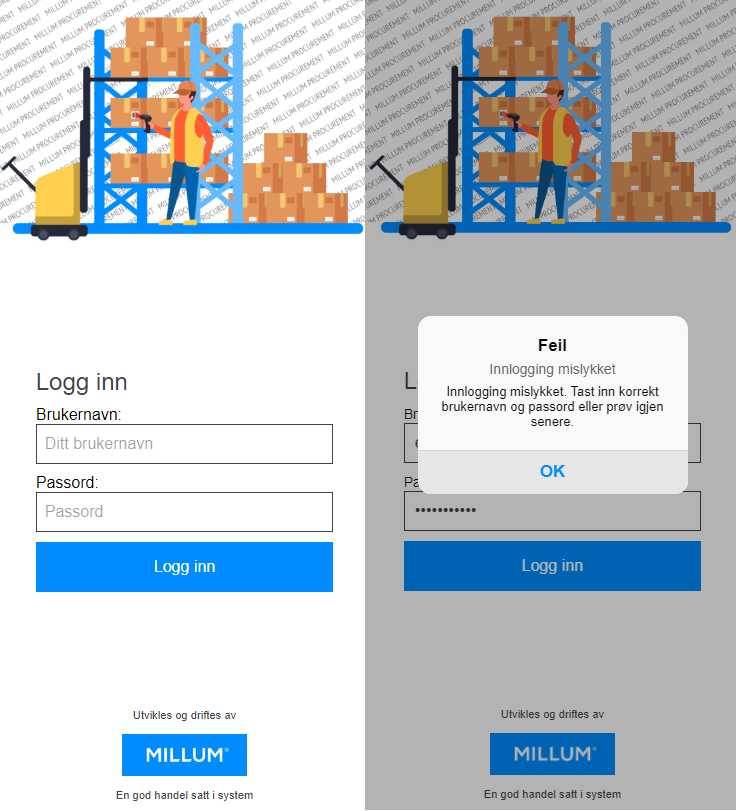
\includegraphics[width=100mm]{figures/BilderLøsning/Login.PNG}
    \caption{Login-siden(t.v). Feil under innlogging (t.h).}
\end{figure}


Når man har lastet ned og åpnet applikasjonen møter man innloggingsiden. Her kan man logge inn med samme bruker som i Millum Procurement, men har ikke mulighet til å opprette ny bruker. Det er rettighetsstyrt av kundene hvem som har anledning til å opprette og redigere brukere, og dette gjøres i et eget system i Millum Procurement. 


Dersom brukerdetaljene ikke stemmer eller andre feil oppstår gir vi vanlige feilmeldinger som ``feil brukernavn eller passord`` eller ``prøv igjen senere``.

\subsection{\textbf{Feil etter innlogging}}
Når brukeren har logget seg inn presenteres en av to mulige visninger basert på om brukeren har delegerte varetellinger eller at tjenesten ikke klarer å innhente data fra API'et til Millum.

\begin{figure}[H] 
    \centering
    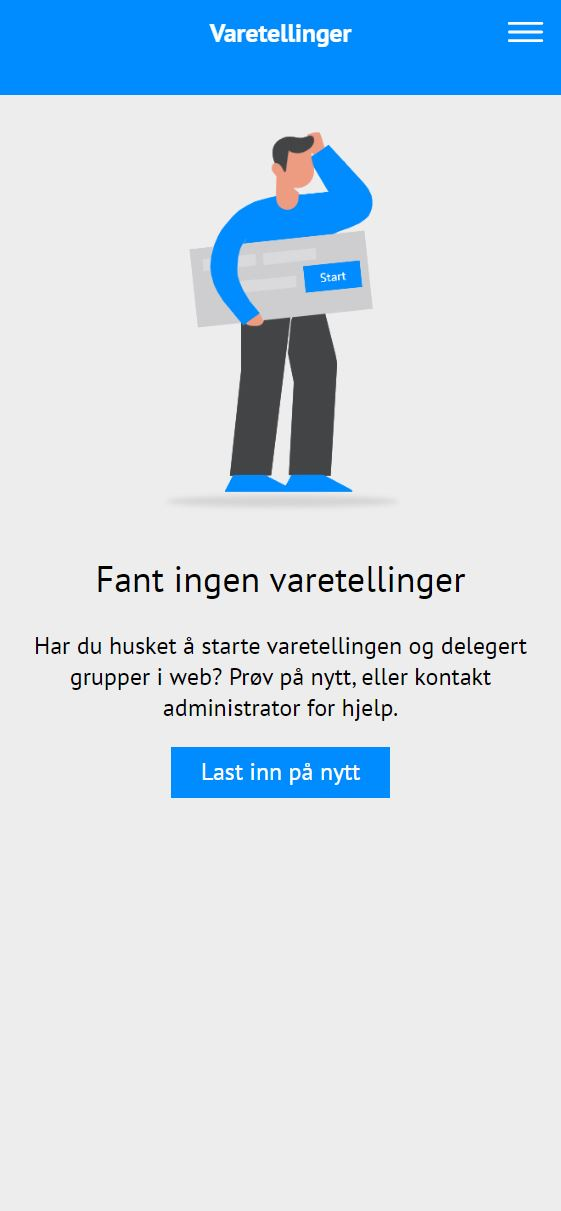
\includegraphics[width=50mm]{figures/BilderLøsning/Ingen_varetellinger.JPG}
    \caption{Skjermdump av ``Ingen varetellinger``}
    \label{Ingen_varetellinger}
\end{figure}

Om bruker får fremvist bildet (\textbf{\ref{Ingen_varetellinger}}), og knappen ``\textbf{Last inn på nytt}`` ikke bringer bruker videre får brukeren en hjelpetekst om mulige feil. Eksempler på dette kan være:

\begin{itemize}
  \item Brukeren har ingen aktive varetellinger.
  \item Eieren av varetellingen har ikke tilgjengeliggjort varetellingen for brukeren (delegert).
  \item Tjenesten som sender varetellingsdata er utilgjengelig.
\end{itemize}

\subsection{\textbf{Introduksjon}}
\begin{figure}[H] 
    \centering
    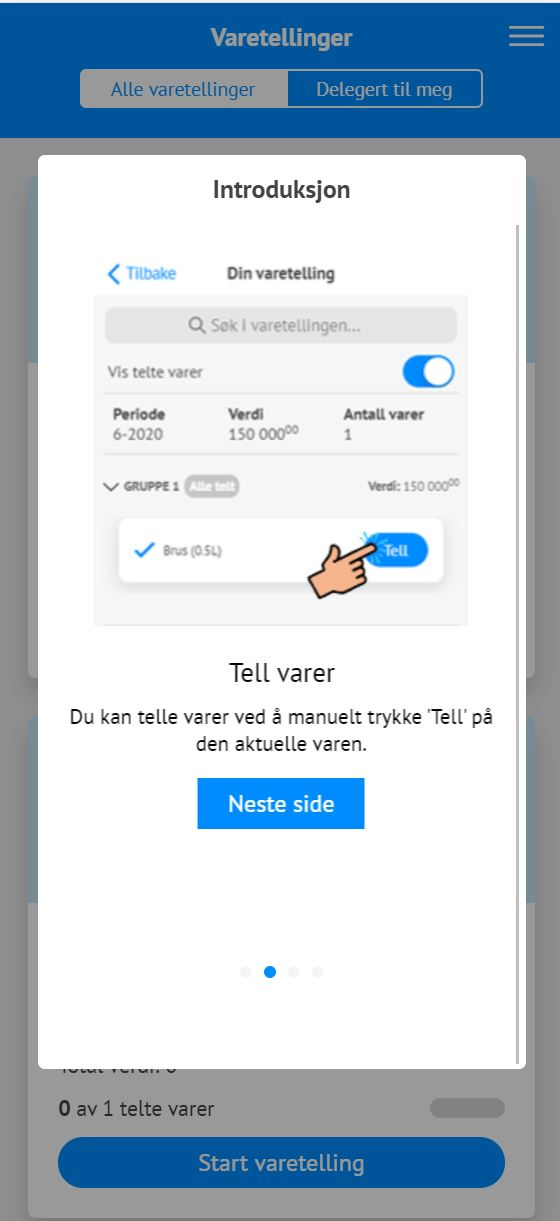
\includegraphics[width=50mm]{figures/BilderLøsning/Wizard.JPG}
    \caption{Visning av wizard}
    \label{Wizard}
\end{figure}

Første gang brukeren logger inn i løsningen vil de bli presentert med en fem-stegs introduksjon til hvordan man gjennomfører varetellingen (\textbf{\ref{Wizard}}), heretter kalt ``Wizard``. Disse fem stegene beskrives med tekst og suppleres med bilder som viser hvordan handlingen utføres. Man kan når som helst avbryte introduksjonen ved å trykke utenfor dialogvinduet.

Etter en kort innføring er brukeren inne på oversiktssiden. Denne visningen er oversikten over brukerens egne varetellinger og de varetellingene som brukeren har blitt delegert av en annen i organisasjonen. Når brukeren trykker ``\textbf{Start varetelling}`` vil det i tillegg gis et valg om i hvilken gruppe bruker ønsker å starte å telle varer i, som vist i \textbf{\ref{DashboardStart}}.. Hensikten med denne funksjonaliteten er at mange av organisasjonene grupperer varene kategorisk i egne varelokasjoner. Det er derfor mer hensiktsmessig å ha skiller mellom lokasjonene så man kan gjøre seg helt ferdig med en lokasjon før man teller videre i en annen.

\begin{figure}[H] 
    \centering
    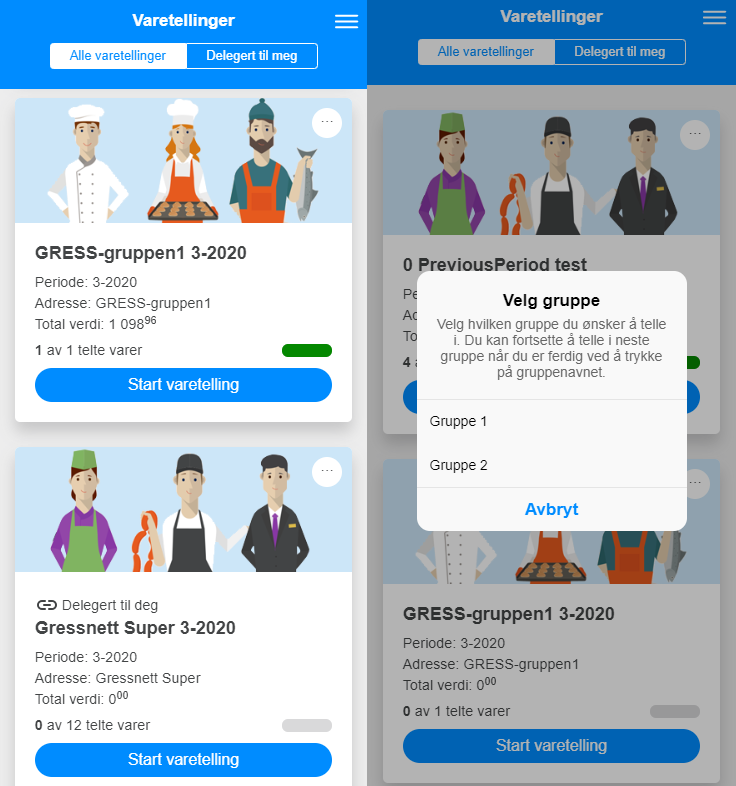
\includegraphics[width=100mm]{figures/BilderLøsning/DashboardStart.png}
    \caption{Dashboard (t.v). Bruker trykker start varetelling (t.h).}
    \label{DashboardStart}
\end{figure}

Dersom eieren av varetellingen \textit{ikke} strukturerer varetellingen med forskjellige grupper vil alle varer bli liggende under \textit{ugruppert}. Dette er noe vi ikke ønsker ettersom ikke flere brukere kan bli delegert samme gruppe.  

\begin{figure}[H] 
    \centering
    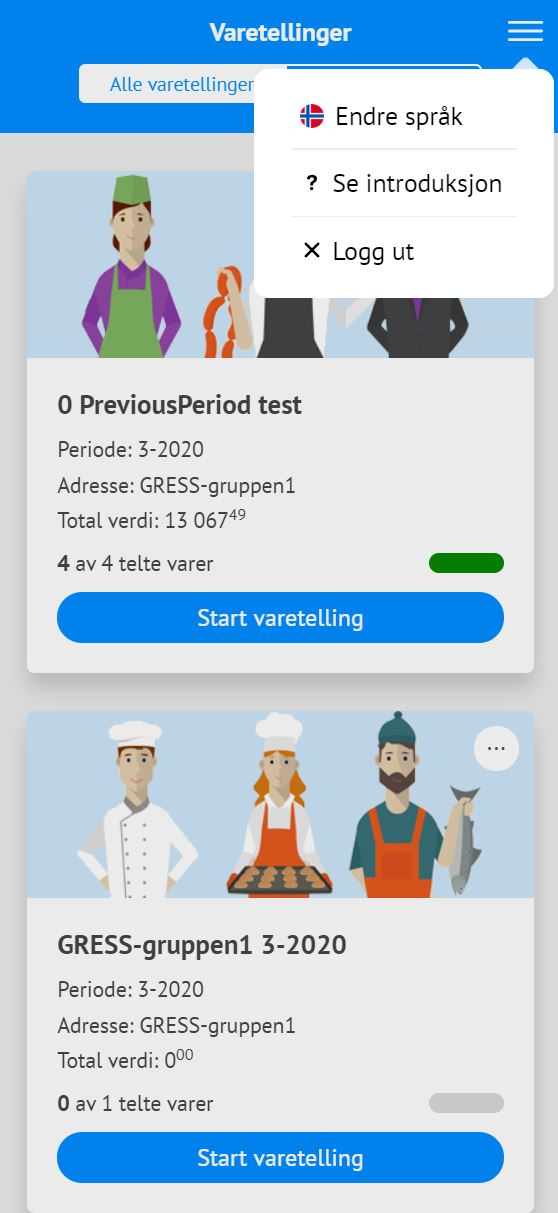
\includegraphics[width=75mm]{figures/BilderLøsning/Hamburger.JPG}
    \caption{Hamburgermeny på oversiktsiden}
\end{figure}

På høyresiden av toppmenyen ligger en nedtrekksmeny. Ved trykke på denne menyen vil man få tre valg:
\begin{itemize}
    \item \textbf{Velge et annet språk.} Når man logger inn hentes valgt språk fra webløsningen, dette valget huskes bare til du logger ut av applikasjonen. Det er mulig å velge mellom norsk, svensk, dansk og engelsk.
    \item \textbf{Se introduksjonen på nytt.}
    \item \textbf{Logge ut.} Sletter all varetellingsdata på mobilenheten.
\end{itemize} 


\subsection{\textbf{Gjennomføring av en varetelling}}

\begin{figure}[H] 
    \centering
    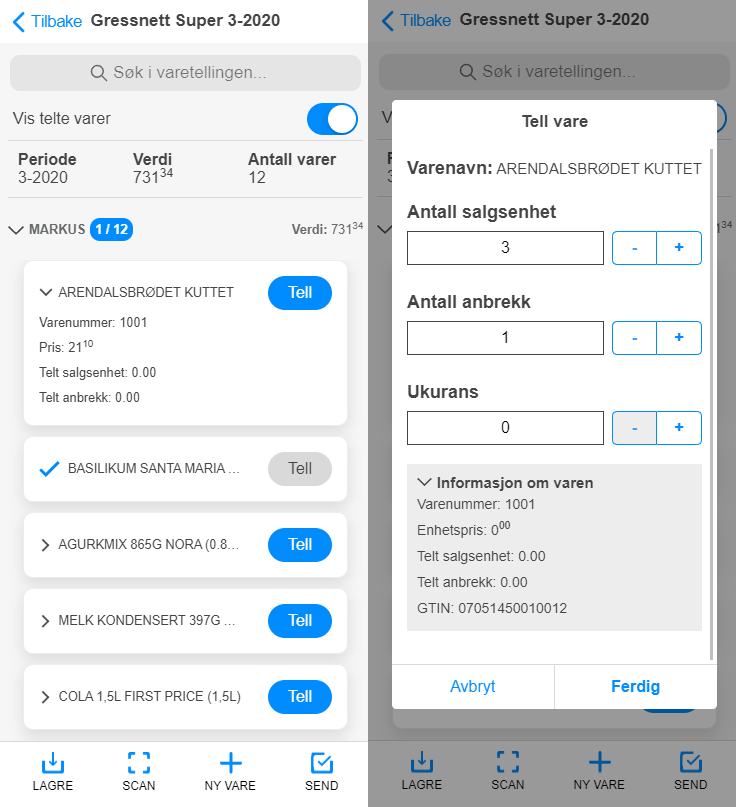
\includegraphics[width=100mm]{figures/BilderLøsning/VaretellingOgTellVare.png}
    \caption{Visning under varetelling (t.v). Når bruker trykker ``Tell`` (t.h).}
\end{figure}

Når brukeren har valgt rett varetelling kan arbeidet starte. Som vist i figur \textbf{\ref{DashboardStart}} vil den gruppen som bruker velger å starte i være åpen, mens de andre gruppene vil være lukket. Helt øverst har bruker mulighet til å søke etter varer på tvers av sine grupper. Dette er én av flere måter brukeren kan finne frem til rett vare dersom varetellingen inneholder mange varer. Når du har telt varene oppdateres verdi i gruppe og totalt for varetellingen øverst, hvor du også kan se antall varer og vise telte varer ettersom de skjules når de er telt. 

Hvis man ønsker å forkaste endringer eller av andre grunner forlate varetellingen kan man benytte tilbake-knappen i headeren som gir deg en advarsel som vist i \textbf{\ref{Ulagrede_endringer}}

\begin{figure}[H] 
    \centering
    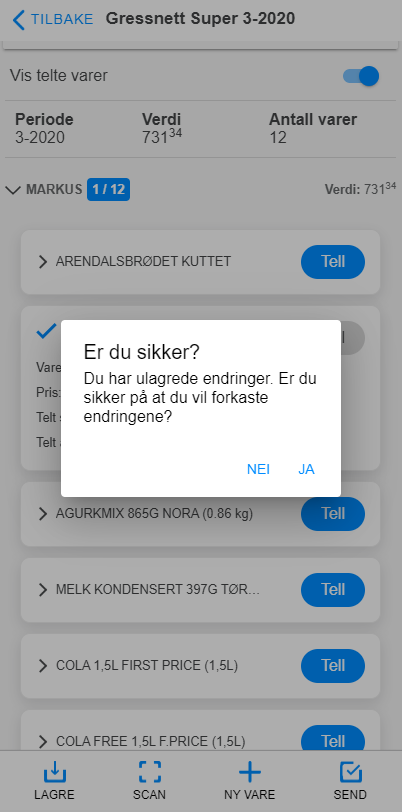
\includegraphics[width=75mm]{figures/BilderLøsning/ulagretVaretelling.PNG}
    \caption{Varsel om ulagrede endringer.}
    \label{Ulagrede_endringer}
\end{figure}


\begin{figure}[H] 
    \centering
    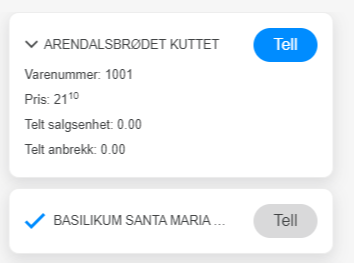
\includegraphics[width=100mm]{figures/BilderLøsning/ikkeTeltogTeltVare.PNG}
    \caption{En vare som ikke er telt (øverst) og telt vare under}
    \label{IkkeTeltOgTeltVare}
\end{figure}

%%Noe om informasjon vi viser under en vare?
Som nevnt vil varene som er telt automatisk skjules, men er likevel tilgjengelig dersom man trykker på ``Vis telte varer``. Vi skiller også visuelt mellom telte og utelte varer med sjekk-ikon og grå knapp. Man har mulighet til å telle nye verdier dersom man oppdager at man har flere av varen.

Nederst på siden er det fire knapper, som vist i \textbf{\ref{Knapper_VT}}.

\begin{figure}[H] 
    \centering
    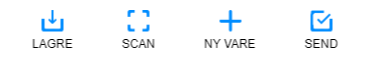
\includegraphics[width=100mm]{figures/BilderLøsning/nedersteKnapper.PNG}
    \caption{De fire knappene nederst under varetellingssiden.}
    \label{Knapper_VT}
\end{figure}

De forskjellig knappene har følgende ansvar:

\begin{itemize}
    \item \textbf{Lagre}, sørger for at alt som er endret på av verdier blir lagret lokalt på enheten.
    \item \textbf{Scan}, åpner strekkodeleseren for scanning av varer.
    \item \textbf{Ny vare}, opprett en egendefinert vare. Mer om dette under \textbf{\ref{Avvik}}
    \item \textbf{Send}. Her kan man levere inn varetellingen til eieren slik at arbeidet kan ferdigstilles. Mer om dette under \textbf{\ref{Innsending}}
\end{itemize}

\subsection{\textbf{Tell vare}} 

\begin{figure}[H] 
    \centering
    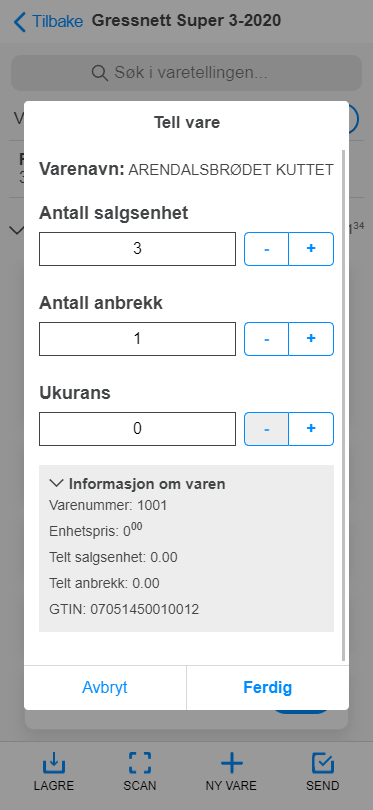
\includegraphics[width=75mm]{figures/BilderLøsning/TellVare.PNG}
    \caption{Visning av vare i tellemodus}
\end{figure}

Ved å lese strekkoden til en vare, eller finne den i varetellingen kan man åpne varen, som gir tilgang til tellefeltene:

\begin{itemize}
    \item \textbf{Antall salgsenhet}. Hva slags slagsenhet varen er leveres av produsent, og kan være f.eks: ``Flaske``, ``Kartong``, ``Glass`` osv.
    \item \textbf{Antall anbrekk}. Dersom varen er en anbrekkvare, eksempelvis leverer produsenten en sekspakning med øl, men man fortsatt ha flere enkeltflasker (anbrekk) igjen på lageret.
    \item \textbf{Antall vekt/volum}. Dersom produsenten oppgir vekt eller volum på varen, f.eks. 10 Kg mel, kan man veie dette for å få riktig verdi. 
    \item \textbf{Ukurans}. Dersom virksomheten har konfigurert det, har man mulighet til å registrere avvik i form av ``ukurans``. Det er for eksempel et knust syltetøyglass.
\end{itemize}

Tilhørende disse tellefeltene er det \textit{Input Steppers} (\textbf{\ref{Universell_utforming}}) som gir brukeren mulighet til å registrere eller justere antall raskt, f.eks. Om man bare har en eller to stykk av varen. 

Avslutningsvis kan man utvide produktinformasjonen dersom man er usikker på om det er riktig vare. Mange produkter har like navn, men f.eks forskjellig vekt - man kan da sikre seg at man teller riktig vare ved å se på varenummer eller GTIN (strekkode).




\subsection{\textbf{Håndtering av avvik}} \label{Avvik}
Brukeren kan oppleve at noen av varene på lageret ikke ligger i varetellingen. Eksempelvis kan sesongvarer eller lignende ikke ligge i handlelistene som ofte brukes som utgangspunkt når varetellingene opprettes, eller at man ikke får treff på en strekkode. Det har vært høyt fokus på å kunne håndtere avvik mens man gjennomfører tellingen slik at man ikke mister flyten og må gjøre ekstra administrative tiltak.

\subsubsection{\textbf{Egendefinerte varer}}
Når varen ikke ligger i varetellingen har du flere muligheter avhengig av om du har internettilgang eller om du leser strekkoden på varen. Du har mulighet til å legge inn en ``egendefinert vare`` (\textbf{\ref{Egendefinert_vare}}). Typisk er dette varer som kanskje ikke handles gjennom handelsløsningen til Millum, eller på andre måter ikke kan hente produktdata fra Millum sine systemer. Vi har fulgt standarden om at påkrevde felter er markert med en rød '*'.

\begin{figure}[H] 
    \centering
    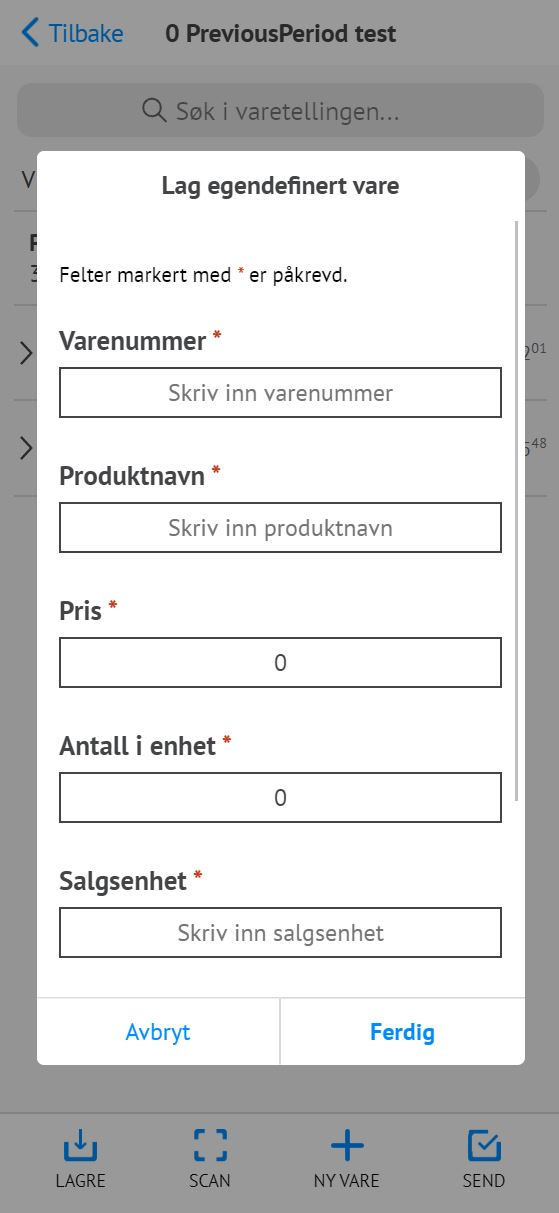
\includegraphics[width=50mm]{figures/BilderLøsning/egendefinert_vare.JPG}
    \caption{Modal for å lage egendefinert vare.}
    \label{Egendefinert_vare}
\end{figure}

\subsubsection{\textbf{Ingen treff på strekkode}}
Om du leser av strekkoden på produktet og ikke får treff kan dette skyldes flere ting. Eksempelvis kan produkter som syltetøy leveres i kartonger med egne strekkoder. Derfor kan produsenten oppgi strekkoden til esken og ikke produktet til leverandøren. En annen årsak er at varen ikke ligger i varetellingen. Du får en sortert liste med handlinger du kan gjøre:
\begin{itemize}
    \item 1. \textbf{Knytte strekkoden til en vare i varetellingen din.} Da vil man få treff på den eksisterende strekkoden og strekkoden du har lest av.
    \item 2. \textbf{Søke etter varer i varekatalogene man har tilgang til.} Da kan man legge inn nye produkter og knytte strekkoden til denne varen i fremtiden. Denne handlingen krever internettilgang og vil gi deg feilmelding om du ikke har dette.
    \item 3. \textbf{Opprette egendefinert vare.}
\end{itemize}

\begin{figure}[H] 
    \centering
    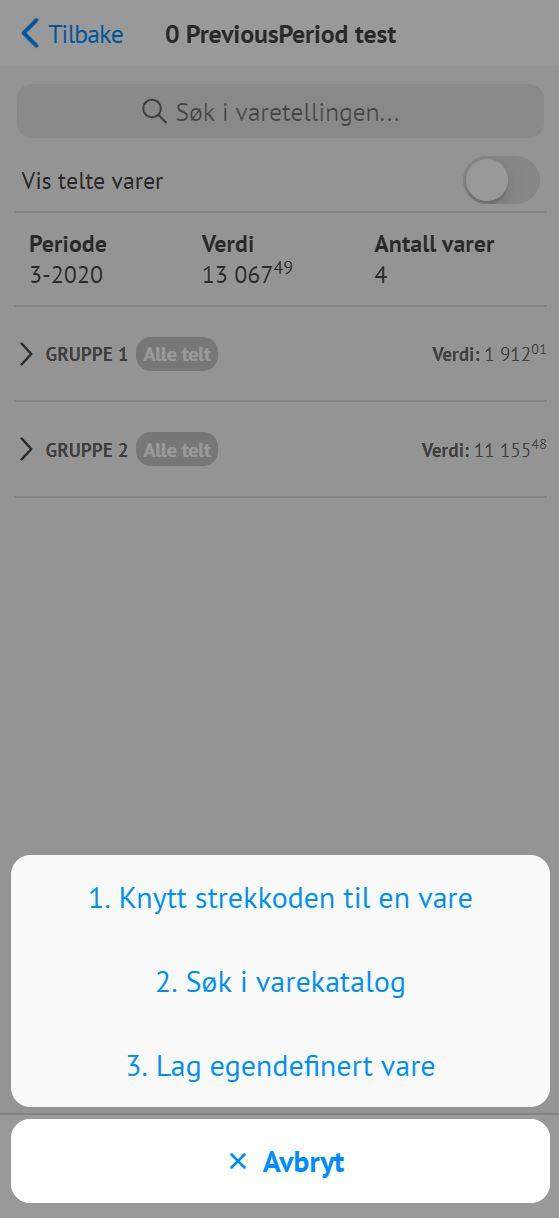
\includegraphics[width=50mm]{figures/BilderLøsning/Ingen_treff_strekkode.JPG}
    \caption{Handlinger når man ikke får treff på strekkoden.}
\end{figure}

%%Eget avsnitt om alle scenarioer? Typ mistet internett på kjølerommet o.l eller bare beskrive rent generelt under "Løsningen"?
\subsection{\textbf{Internettdekning og bruk av applikasjonen offline}}
En av de store utfordringene mange av brukerne står ovenfor ved bruk av digitale hjelpemidler ved gjennomføring av en varetelling er at det kan være dårlig eller ingen internettdekning på varelagrene. Vi har derfor utviklet funksjonalitet for å hjelpe brukeren med å gjennomføre varetellingen selv om man ikke har dekning.

\subsubsection{\textbf{Prosess}}
Man må alltid ha dekning for å kunne logge inn og laste ned varetellingene. Så snart dette er gjort lagres varetellingen lokalt på mobilenheten og du vil ha mulighet til å telle varer, håndtere avvik og lignende. Dersom handlingen du prøver å gjøre krever internettilgang vil du bli varslet om at man må ha internettforbindelse for å fullføre handlingen.

\subsubsection{\textbf{Håndtering av avvik offline}}
Som nevnt i \textbf{\ref{Avvik}} har man flere muligheter for å håndtere avvik. Dette begrenses noe når man er offline, men kort oppsummert har man mulighet til å knytte strekkoden til en eksisterende vare i varetelling, eller å opprette egendefinert vare.

\section{\textbf{Innsending}} \label{Innsending}

\begin{figure}[H] 
    \centering
    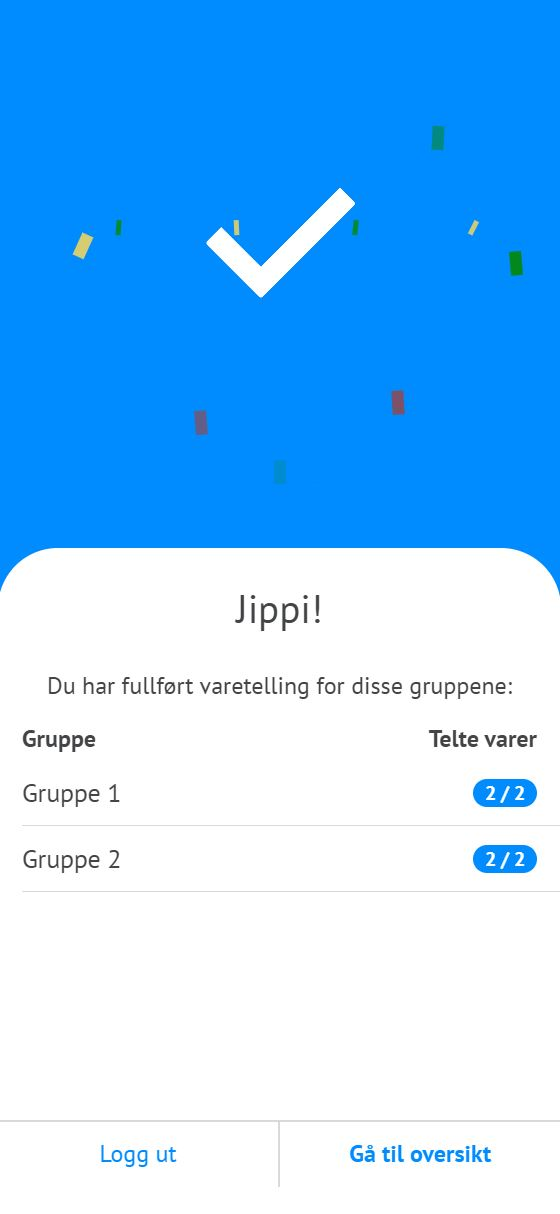
\includegraphics[width=50mm]{figures/BilderLøsning/Levert_varetelling.JPG}
    \caption{Sammendrag av fullført varetelling.}
    \label{Levert_varetelling}
\end{figure}

Det avsluttende steget i varetellingen for brukerens del er å sende inn sin del av varetellingen, og brukeren blir presentert av visningen under figur \textbf{\ref{Levert_varetelling}}. Ved å gjøre dette leverer man tilbake varetellingen til eieren og mister tilgang. Du vil derfor bli presentert med en kort oppsummering av grupper du har levert inn og valget om å logge ut eller gå til oversiktsiden. 

\section{\textbf{Akseptansetest}}

Her kommer akseptansetesten hehehe

